
%(BEGIN_QUESTION)
% Copyright 2009, Tony R. Kuphaldt, released under the Creative Commons Attribution License (v 1.0)
% This means you may do almost anything with this work of mine, so long as you give me proper credit

The {\it Nernst equation} finds application in many different chemical analyzer technologies, not just pH measurement.  One of these analytical technologies is {\it oxygen concentration} in mixed gas streams, such as the exhaust from a combustion process where oxygen content is usually maintained at about 2\% (instead of the normal 20.9\% oxygen concentration of Earth's atmosphere).  A common oxygen sensor is made of a ``sandwich'' of platinum electrodes on either side of a solid zirconium oxide membrane.  One side of this electrochemical cell is exposed to the exhaust gas (process), while the other side is exposed to heated air which serves as a reference:

$$\includegraphics[width=15.5cm]{i00685x01.eps}$$

Voltage output by the cell is predicted by the Nernst equation:

$$V = {{R T} \over {nF}} \ln \left({C_1 \over C_2}\right)$$

Explain why temperature must be precisely controlled at the zirconium oxide cell in order to maintain accurate calibration of this instrument.  Also, identify the relationship between measured oxygen content and cell output voltage (i.e. is voltage {\it directly} or {\it inversely} related to oxygen content?) for applications such as furnace exhaust oxygen measurement.

\vfil

\underbar{file i00685}
\eject
%(END_QUESTION)





%(BEGIN_ANSWER)

This is a graded question -- no answers or hints given!

%(END_ANSWER)





%(BEGIN_NOTES)

Voltage is a function of oxygen concentration {\it and} temperature in this sensor, so it is critical to maintain a stable temperature in order that the voltage-to-oxygen relationship be predictable.

\vskip 10pt

Voltage is {\it inversely proportional} to oxygen concentration at levels below atmospheric (20.9\%), because the amount of voltage produced by the zirconium oxide cell is proportional to the {\it difference} in oxygen concentration on either side of the cell.  As process O$_{2}$ concentration increases toward atmospheric (20.9\%), that difference grows smaller and the voltage approaches zero.  As the process oxygen concentration decrease toward zero, the differential concentration across the cell grows larger, producing more voltage.

%INDEX% Chemistry, electro-: Nernst equation
%INDEX% Measurement, analytical: oxygen (high temperature)

%(END_NOTES)


